\section{Methodology}

\subsection{Overview of the traditional and bonus pipelines}

The implementation separates a \textbf{traditional path} (configurable preprocessing $\rightarrow$ feature extraction to disk $\rightarrow$ classical classifiers $\rightarrow$ evaluation) from a \textbf{bonus deep-learning path} (Word2Vec + BiLSTM on the same preprocessed text). Configurations are encoded by dataclasses (\texttt{PreprocessConfig}, \texttt{ExperimentConfig}). Results are cached by dataset, preprocessing tag, and method. Random seeds are fixed to 42.

\begin{figure}[H]
\centering
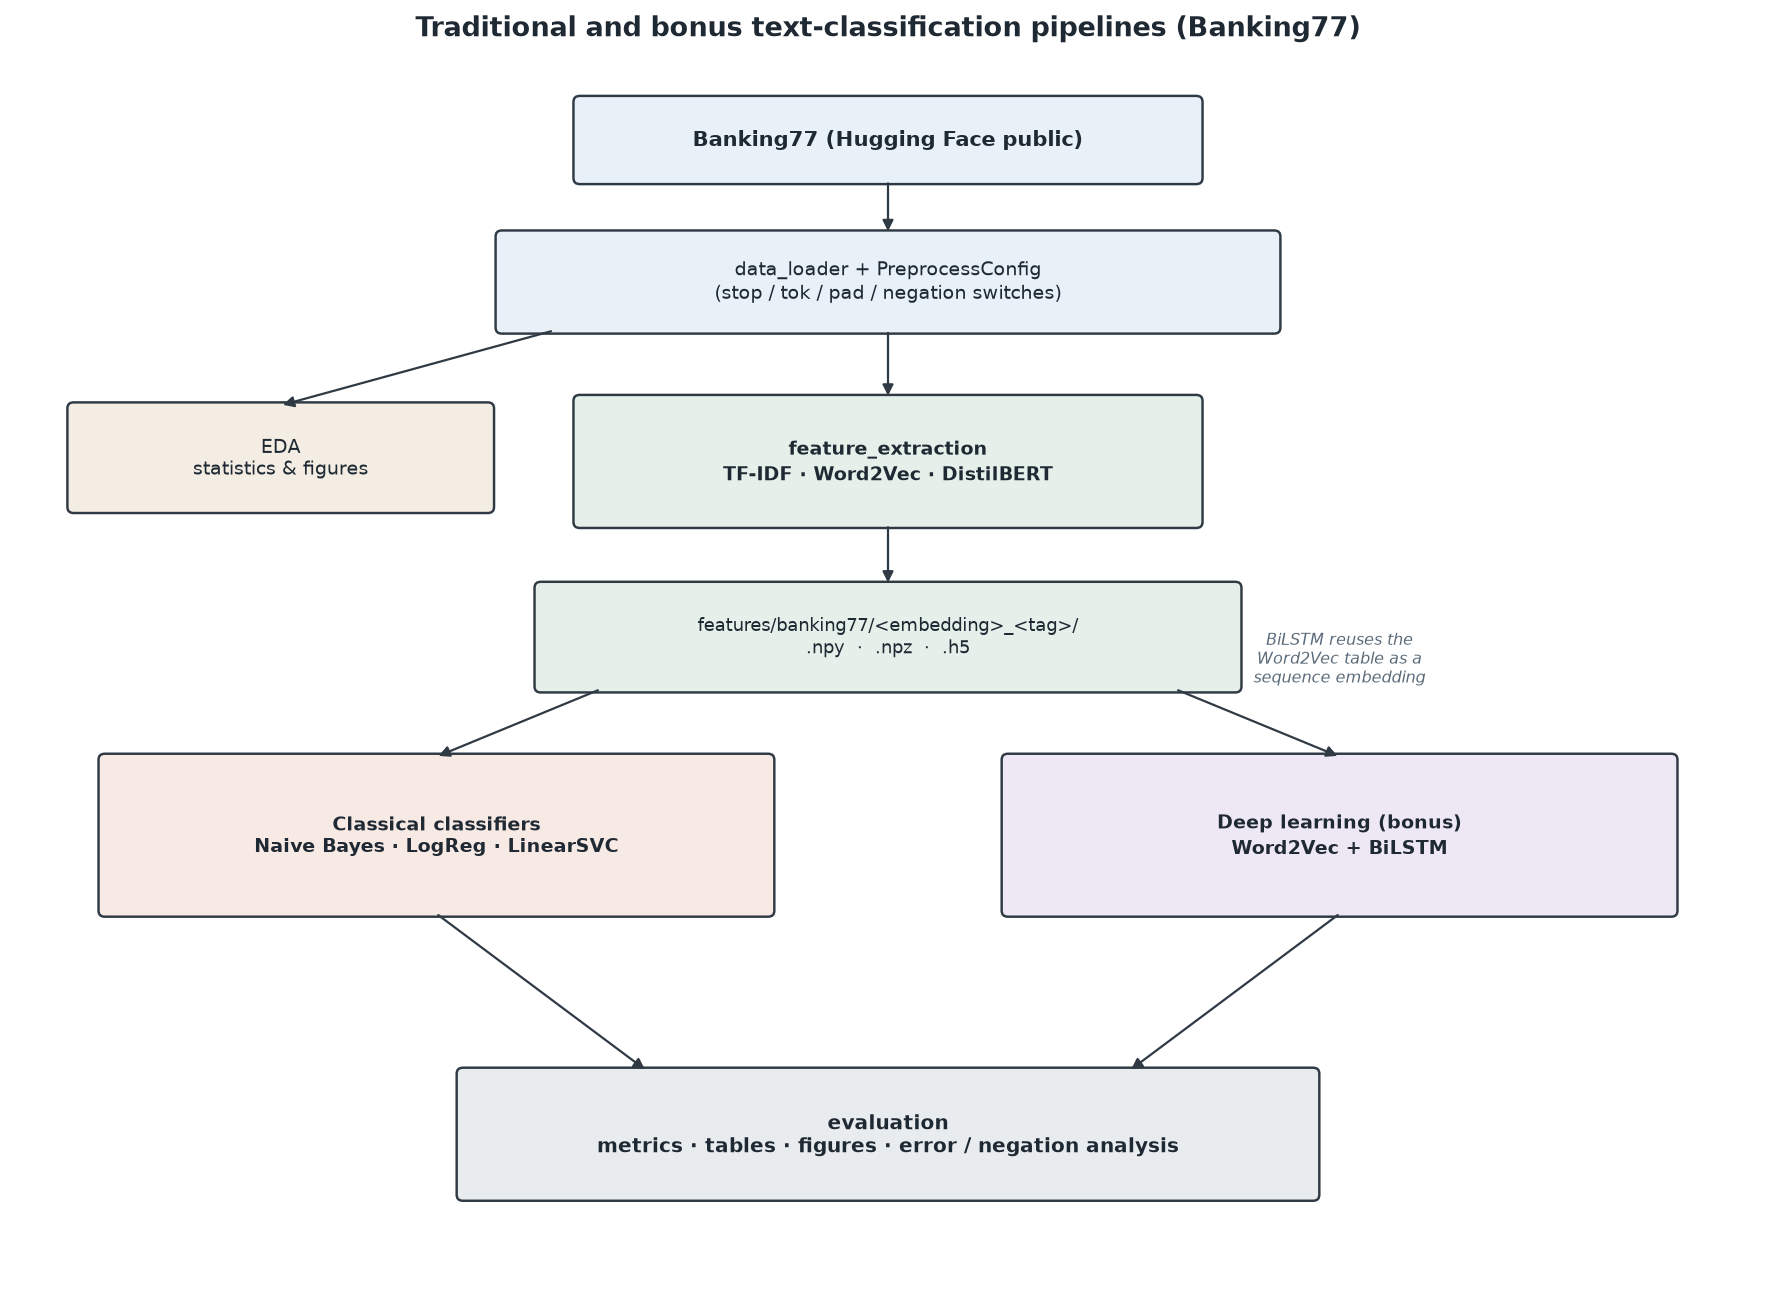
\includegraphics[width=0.95\textwidth]{pipeline_overview.png}
\caption{Overview of the traditional and bonus text-classification pipelines on Banking77.}
\end{figure}

\subsection{Preprocessing}

All text is lower-cased and stripped of HTML, URLs, and related artefacts. Four Boolean switches control the remainder:

\begin{table}[H]
\centering
\caption{Boolean preprocessing switches.}
\small
\begin{tabular}{@{}p{3.2cm}p{5.2cm}p{5.5cm}@{}}
\toprule
Switch & Off & On \\
\midrule
\texttt{stop\_word\_removal} & retain all tokens & remove scikit-learn \texttt{ENGLISH\_STOP\_WORDS} \\
\texttt{tokenization} & whitespace unigrams / whole-word lookup & regex tokens + bigrams for TF-IDF; WordPiece for DistilBERT \\
\texttt{padding} & truncate to 10 tokens; no masking & pad/truncate to the 95th-percentile length with masks \\
\texttt{negation\_marking} & unchanged text & join negation cue with next token (\texttt{not\_arrived}) \\
\bottomrule
\end{tabular}
\end{table}

The default for the main comparison is \texttt{sw0\_tok1\_pad1\_neg0}. Padding is not applicable to bag-of-words / TF-IDF models.

\subsection{Feature extraction and persistence}

\begin{table}[H]
\centering
\caption{Feature extractors used in the default experiment grid.}
\small
\begin{tabular}{@{}llp{7.2cm}@{}}
\toprule
Key & Family & Representation \\
\midrule
\texttt{tfidf} & traditional & \texttt{TfidfVectorizer} (sublinear TF, max 25k features, \texttt{min\_df}=2), uni+bigrams \\
\texttt{word2vec} & static & skip-gram Word2Vec on the training split (300-d); mean-pooled documents \\
\texttt{distilbert} & modern & frozen DistilBERT; masked mean pool (768-d) \\
\bottomrule
\end{tabular}
\end{table}

Vectorizers and Word2Vec are fit on training data only. Each feature directory stores dense \texttt{.npy} or sparse \texttt{.npz} arrays, labels, a consolidated \texttt{features.h5}, and \texttt{meta.json}. BoW remains available as a plug-in embedding type in the module API but is not part of the default experiment grid.

\subsection{Classical classifiers}

\begin{table}[H]
\centering
\caption{Classical classifiers on sparse and dense inputs.}
\small
\begin{tabular}{@{}lll@{}}
\toprule
Classifier & Sparse input (TF-IDF) & Dense input (embeddings) \\
\midrule
Naive Bayes & MultinomialNB ($\alpha=0.5$) & GaussianNB \\
Logistic regression & $C=2.0$, balanced, L-BFGS & StandardScaler + same \\
Linear SVM & LinearSVC ($C=1.0$, balanced) & L2 Normalizer + same \\
\bottomrule
\end{tabular}
\end{table}

Dense SVM inputs are L2-normalised for stable convergence. SVM probabilities use Platt scaling (3-fold).

\subsection{Bonus deep-learning model}

The bonus component is \textbf{Word2Vec + BiLSTM}: the same skip-gram table used for mean pooling initialises a trainable embedding layer; a one-layer bidirectional LSTM (hidden size 192) produces the document representation. Early stopping monitors a stratified 10\% validation split of the training set (patience 2, up to 7 epochs).

\subsection{Evaluation protocol}

Models train on the official training split and are evaluated once on the held-out test split. We report accuracy, macro-averaged precision, recall, and F1, and calibration scores
\begin{equation*}
\mathrm{Brier}
  = \frac{1}{N}\sum_{i=1}^{N}\sum_{k=1}^{K}\bigl(p_{ik}-y_{ik}\bigr)^{2},
\qquad
\mathrm{ECE}
  = \sum_{b=1}^{15}\frac{|B_b|}{N}\bigl|\mathrm{acc}(B_b)-\mathrm{conf}(B_b)\bigr|.
\end{equation*}
